%%%%%%%%%%%%%%%%%%%%%%%%%%%%%%%%%%%%%%%%%%%%%%%%%%%%%%%%%%%

\chapter{Modello del sistema - gruppo 2 - notifiche}
\label{ref:modSistemaGruppo2-notifiche}

\section{Attori}

<Gli attori di Notifiche sono in comune agli altri gruppi>.

\section{Scenari}

\subsection{Apertura finestra di prenotazione per l’appello d’esame}

Il sistema invia una notifica push allo studente Angelo Gino Varrati, identificato per mezzo di matricola 123456, in concomitanza con l’apertura della finestra di prenotazione dell’esame di “Ingegneria del Software” del Prof. Fausto Fasano, in quanto ancora da sostenere e presente all’interno della propria carriera.

\subsection{Chiusura finestra di prenotazione per l’appello d’esame}

Il sistema invia una notifica push alla studentessa Giuseppina Mazzocco, identificata per mezzo di matricola 789101, poco prima della chiusura della finestra di prenotazione all’esame di “Ingegneria del Software” del Prof. Fausto Fasano, in quanto ancora da sostenere e presente all’interno della propria carriera.

\subsection{Verbalizzazione esame}

Il sistema invia una notifica push alla studentessa Martina Buro, identificata per mezzo di matricola 234567, in occasione della verbalizzazione dell’esame di “Ingegneria del Software” del Prof. Fausto Fasano, sostenuto in data 28/02/2019 riportando votazione pari a 28.

\subsection{Avviso tasse}

All’apertura del periodo di pagamento di un importo di tasse universitarie, tale evento verrà notificato all’utente per mezzo di una notifica push.

\subsection{Sospensione lezione}

Il sistema invia una notifica push allo studente Angelo Gino Varrati, identificato per mezzo di matricola 123456, in occasione della sospensione della lezione di “Ingegneria del Software” del Prof. Fausto Fasano prevista per il giorno 19/03/2019.

\section{Casi d'uso}

\subsection{Apertura finestra di prenotazione all’appello d’esame}

Vedi Tabella~\vref{tab:caso-duso-apertura-finestra-esame}.

\begin{table}
%\normalsize % Dimensione testo normale
\small % Dimensione testo piccola
%\footnotesize % Dimensione testo piccolissima
%\scriptsize % Dimensione del testo ulteriormente più piccola
\caption{Tabella caso d'uso - Apertura finestra di prenotazione all'appello d'esame} % Didascalia tabella
\label{tab:caso-duso-apertura-finestra-esame} % Etichetta per riferimenti incrociati
\begin{tabular}{| p{\useCaseLeft} | p{\useCaseNum} | p{\useCaseTwoCol} | p{\useCaseTwoCol} |}
	\hline
	\textbf{Nome caso d'uso} & \multicolumn{3}{p{\useCaseMulticol} |}{\textbf{Apertura finestra di prenotazione appello d’esame.}} \\
	\hline
	\textbf{Attori partecipanti} & \multicolumn{3}{p{\useCaseMulticol} |}{Inizializzato da Firebase. Partecipa Studente.} \\
	\hline
	\textbf{Condizioni d'ingresso} & \multicolumn{3}{p{\useCaseMulticol} |}{Connessione ad Internet.} \\
	\hline
	\textbf{Flusso degli eventi} & \textbf{\#} & \textbf{Studente} & \textbf{Firebase} \\
	\hline
	\textbf{} & \textbf{1} & \textbf{} & Invia una notifica. \\
	\hline
	\textbf{} & \textbf{2} & Visualizza la notifica. & \textbf{} \\
	\hline
	\textbf{Eccezioni} & \multicolumn{3}{p{\useCaseMulticol} |}{Lo Studente ha disabilitato la ricezione delle notifiche.} \\
	\hline
	\textbf{Condizioni d'uscita} & \multicolumn{3}{p{\useCaseMulticol} |}{Lo studente visualizza la notifica.} \\
	\hline
\end{tabular}
\end{table}

\subsection{Chiusura finestra di prenotazione all’appello d’esame.}

Vedi Tabella~\vref{tab:caso-duso-chiusura-finestra-esame}.

\begin{table}
%\normalsize % Dimensione testo normale
\small % Dimensione testo piccola
%\footnotesize % Dimensione testo piccolissima
%\scriptsize % Dimensione del testo ulteriormente più piccola
\caption{Tabella caso d'uso - Chiusura finestra di prenotazione all'appello d'esame} % Didascalia tabella
\label{tab:caso-duso-chiusura-finestra-esame} % Etichetta per riferimenti incrociati
\begin{tabular}{| p{\useCaseLeft} | p{\useCaseNum} | p{\useCaseTwoCol} | p{\useCaseTwoCol} |}
	\hline
	\textbf{Nome caso d'uso} & \multicolumn{3}{p{\useCaseMulticol} |}{\textbf{Chiusura finestra di prenotazione all'appello d'esame}} \\
	\hline
	\textbf{Attori partecipanti} & \multicolumn{3}{p{\useCaseMulticol} |}{Inizializzato da Firebase. Partecipa Studente.} \\
	\hline
	\textbf{Condizioni d'ingresso} & \multicolumn{3}{p{\useCaseMulticol} |}{Connessione ad Internet.} \\
	\hline
	\textbf{Flusso degli eventi} & \textbf{\#} & \textbf{Studente} & \textbf{Firebase} \\
	\hline
	\textbf{} & \textbf{1} & \textbf{} & Invia una notifica. \\
	\hline
	\textbf{} & \textbf{2} & Riceve la notifica. & \textbf{} \\
	\hline
	\textbf{Eccezioni} & \multicolumn{3}{p{\useCaseMulticol} |}{Lo Studente ha disabilitato la ricezione delle notifiche.} \\
	\hline
	\textbf{Condizioni d'uscita} & \multicolumn{3}{p{\useCaseMulticol} |}{Lo studente visualizza la notifica.} \\
	\hline
\end{tabular}
\end{table}

\section{Diagrammi dei casi d'uso}

Inserire immagine del diagramma. Le immagini vanno caricate nella cartella imgs, va inserito il path corrispondente (nomefile.estensione) dopo il tag includegraphics e va cambiata la descrizione dell'immagine (caption) con un'etichetta opportuna. Sostituire l'immagine file-comuni-ai-gruppi/useCaseEsempio.png con quella desiderata.

\begin{figure}
	\centering
	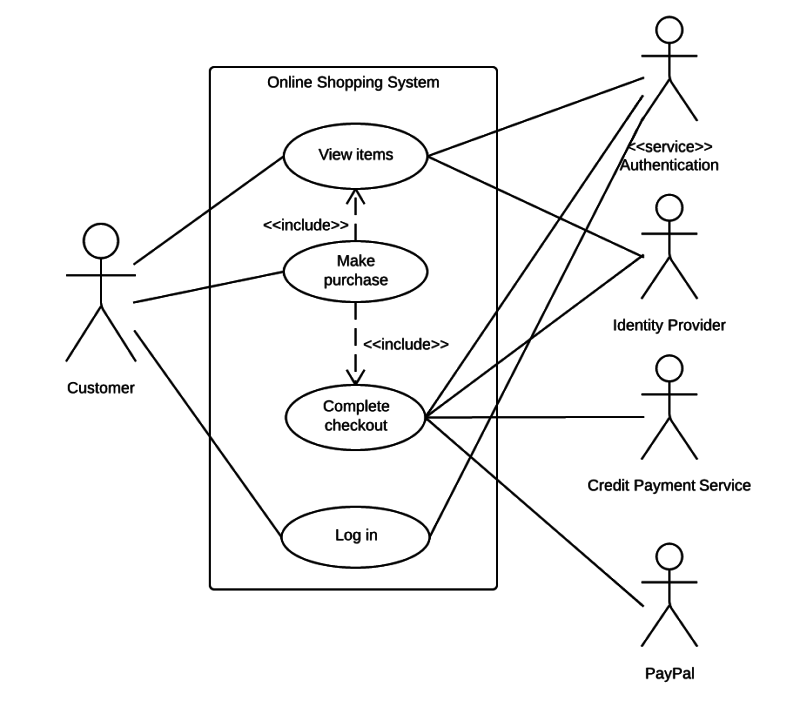
\includegraphics[height=3in]{imgs/file-comuni-ai-gruppi/useCaseEsempio.png}
	\caption{Inserire descrizione}
	\label{fig:prova}
\end{figure}

\section{Diagrammi di sequenza}

Inserire immagine del diagramma. Le immagini vanno caricate nella cartella imgs, va inserito il path corrispondente (nomefile.estensione) dopo il tag includegraphics e va cambiata la descrizione dell'immagine (caption) con un'etichetta opportuna. Sostituire l'immagine file-comuni-ai-gruppi/useCaseEsempio.png con quella desiderata.

\begin{figure}
	\centering
	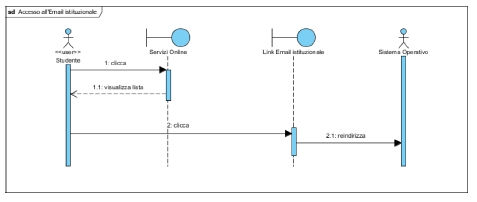
\includegraphics[height=3in,width=5in]{imgs/file-comuni-ai-gruppi/SequenceDgEsempio.png}
	\caption{Inserire descrizione}
	\label{fig:prova}
\end{figure}

\section{Diagrammi delle attività}

Inserire immagine del diagramma. Le immagini vanno caricate nella cartella imgs, va inserito il path corrispondente (nomefile.estensione) dopo il tag includegraphics e va cambiata la descrizione dell'immagine (caption) con un'etichetta opportuna. Sostituire l'immagine file-comuni-ai-gruppi/useCaseEsempio.png con quella desiderata.

\begin{figure}
	\centering
	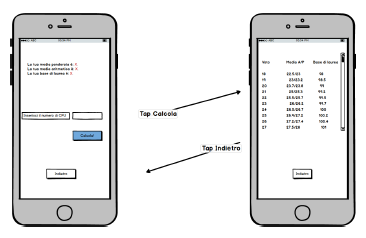
\includegraphics[height=3in,width=5in]{imgs/file-comuni-ai-gruppi/ActivityDgEsempio.png}
	\caption{Inserire descrizione}
	\label{fig:prova}
\end{figure}

\clearpage